\documentclass[10pt]{article}
\usepackage[right=2cm,left=2cm,top=2cm,bottom=3cm]{geometry}
\usepackage[utf8]{inputenc}
\usepackage[spanish]{babel}
\usepackage{amsmath}
\usepackage{color}
\usepackage{listings}
\usepackage{graphicx}
%\usepackage{multicol}

%COLORES CODIGO
\definecolor{gray97}{gray}{.97}
\definecolor{gray75}{gray}{.75}
\definecolor{gray45}{gray}{.45}
\definecolor{claregreen}{RGB}{4,180,95}
\definecolor{darkblue}{rgb}{0.0,0.0,0.6}


\lstset{ frame=Ltb,
     framerule=0pt,
     aboveskip=0.5cm,
     framextopmargin=3pt,
     framexbottommargin=3pt,
     framexleftmargin=0.4cm,
     framesep=0pt,
     rulesep=.4pt,
     backgroundcolor=\color{gray97},
     rulesepcolor=\color{black},
     %
     stringstyle=\ttfamily,
     showstringspaces = false,
     basicstyle=\small\ttfamily,
     commentstyle=\color{gray45},
     keywordstyle=\bfseries,
     %
     numbers=left,
     numbersep=15pt,
     numberstyle=\tiny,
     numberfirstline = false,
     breaklines=true,
   }

% minimizar fragmentado de listados
\lstnewenvironment{listing}[1][]
   {\lstset{#1}\pagebreak[0]}{\pagebreak[0]}

%LENGUAJE OZ
\lstdefinelanguage{OZ}
{
  morestring=[b]',
  morecomment=[s]{\%}{\%},
  stringstyle=\color{claregreen},
  keywordstyle=\color{blue}\bfseries,
  morekeywords={proc, end, \$},% list your attributes here
  emph={REQUIRED},
  emphstyle=\color{red}
}

%MODO CONSOLA
\lstdefinestyle{consola}
   {basicstyle=\scriptsize\bf\ttfamily,
    backgroundcolor=\color{gray75},
   }




%opening
\title{Simulación de Eventos Discretos.\\ \emph{Informe de Modelo e Implementación.} \\ \textbf{Simulación de Fallas de Máquinas.} }
\author{\textbf{María Andrea Cruz Blandon  0831816.} \\ \textbf{Edgar Andres Moncada 0832294.  }\\ \textbf{Luis Felipe Vargas Rojas 0836342. }}
\date{\today}







\begin{document}
\maketitle

\section{Análisis del Sistema y del Problema.}
\subsection{Descripción del Sistema}
El sistema esta compuesto de un conjunto de maquinas que funcionan en una fabrica, entre las cuales no existe conexión de manera que cada una trabaja independientemente de las otras; estas se mantienen encendidas 8 horas del día, es decir que el rendimiento total semanal se calcula con la formula $8*5*50$ donde 8 son las  horas del dia, 5 son los días de la  semana, y 50 es el número de maquinas que están laborando.\\

Dentro de la fabrica se cuenta con un conjunto de maquinas adicionales que son enviadas a trabajar si alguna de las maquinas presenta una falla. Tambien se cuenta con personal de mantenimiento, que se encargan de reparar las maquinas que puedan fallar; cada empleado puede reparar una maquina al tiempo, en caso de no tener a algun empleado disponible se debe ponerse en espera, y en el momento de que un empleado la reemplace esta se convierte en una maquina adicional.


\subsection{Descripción Gráfica del Sistema}
\begin{center}

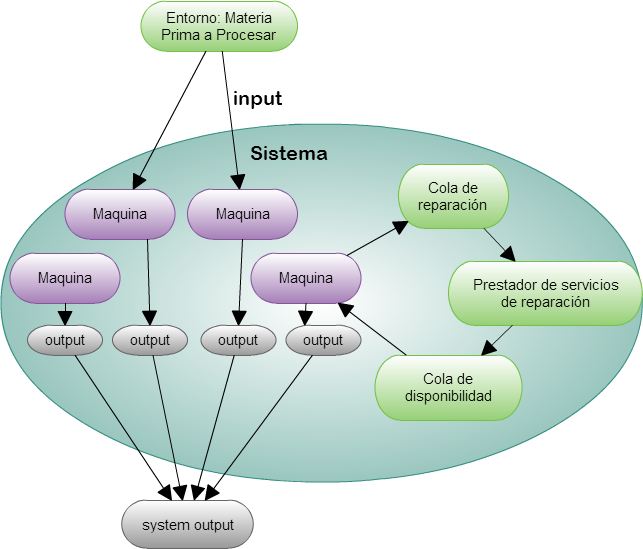
\includegraphics[scale=0.47]{Simulacion.png}

Figura1. \emph{Comportamiento del Sistema}
\end{center}

\subsection{Descripción del Problema}

La fabrica quiere mantener el stock de maquinaria principal en funcionamiento continuo por lo menos en un 96\% o 98\%. El problema que se tiene es que las maquinas son componentes que pueden presentar fallas, y estas afectan de manera general a la producción de la fabrica.\\

Para solucionar este problema la fabrica ha dispuesto de maquinas adicionales dispuestas a suplantar las maquinas que se dañen durante el proceso, que tienen a fallar luego de $16\pm6$ horas, y tambien se cuenta con un equipo de mantenimiento que puede reparar las maquinas que se dañen en aproximadamente $8\pm3$ horas. Sin embargo no siempre son suficientes las maquinas auxiliares y la cantidad de personal para atender las maquinas que fallan y mantener la utilidad requerida de funcionamiento de las 50 maquinas. Por esta razon la fabrica quiere determinar cuantas maquinas adicionales y cuanto personal es el necesario para cumplir la meta.

\section{Modelo de Simulación.}

\subsection{Eventos.}

\begin{itemize}
\item Falla de una maquina.
\item Reparación de una maquina.
\end{itemize}

Diagramas de flujo de los eventos:
\begin{center}

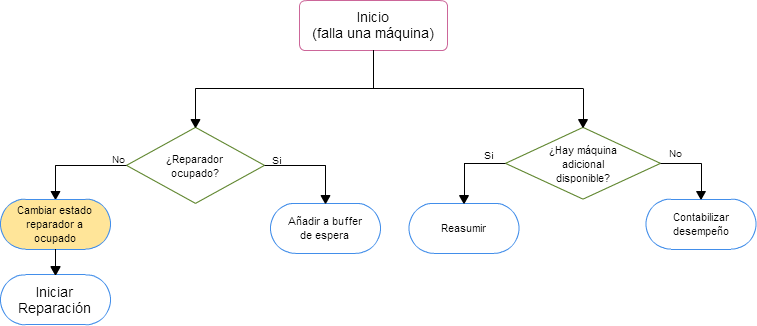
\includegraphics[scale=0.47]{fallaMaquina.png}

Figura2. \emph{Evento: Se presenta una falla en una de las maquina.}
\end{center}
\begin{center}

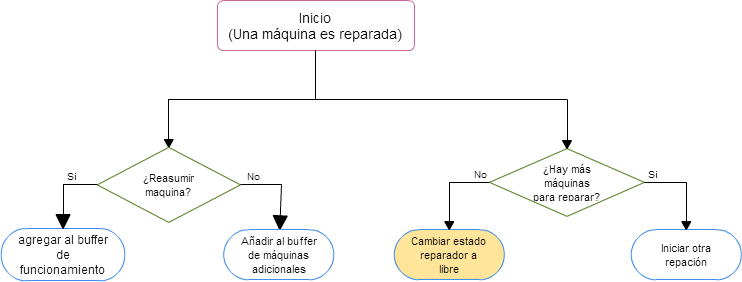
\includegraphics[scale=0.47]{reparar.png}

Figura3. \emph{Evento: Se realiza la reparación de una de las maquinas dañadas.}
\end{center}



\subsection{Reloj de La Simulación}

La unidad de tiempo que se va a emplear es la hora, el reloj va a avanzar de acuerdo al modelo de simulación LEF, donde se almacenan los tiempos de los eventos futuros y se ordenan cronológicamente, así el cambio de estado del reloj  se va a dar por el tiempo del evento más próximo en cada iteración.\\

La simulacion termina cuando:
\begin{enumerate}
\item El reloj del sistema a llegado a un valor indicado.
\item no hay mas eventos futuros en el arreglo.
\end{enumerate}

\subsection{Comportamiento de los Datos.}

\begin{itemize}
\item \textbf{Fallo de una maquina:}
\item \textbf{Reparación de una maquina:}

\end{itemize}



\section{Diseño y Analisis de Escenarios.} 


\section{Implementación del Modelo.}




\section{Conclusiones.}



\end{document}
